\section{Conservative and non-conservative forces}
	Based on the nature of the work done, we can classify different forces into two types:
	\begin{enumerate}
		\item \emph{Conservative force:} A force is said to be conservative if the work done by it in displacing a particle between two arbitrary points depends only on the end points, and is independent of the actual path taken by the particle.
		\begin{itemize}
			\item The net work done in a closed loop is always zero.
			\item The mechanical energy (kinetic energy + potential energy) of the system is always conserved.
			\item Examples of conservative forces:
			\begin{enumerate}
				\item Gravitational force -- moving an object up and down takes or returns the exact same amount of energy, regardless of whether it is lifted straight up or taken by a winding ramp.
				\item Elastic force -- the force exerted by a stretched or compressed ideal spring depends solely on its displacement from the equilibrium position.
				\item Electrostatic force -- the force between two static electric charges depends only on their positions and magnitudes, not how they arrived there.
			\end{enumerate}
		\end{itemize}
		
		\item \emph{Non-conservative force:} A force is said to be non-conservative if the work done by it in displacing a particle between two arbitrary points depends on the end points, as well as on the actual path taken by the particle.
		\begin{itemize}
			\item The net work done in a closed loop is non-zero.
			\item The mechanical energy (kinetic energy + potential energy) of the system is not conserved, but dissipated into other forms such as sound and heat.
			\item Most non-conservative forces are \emph{velocity-dependent}.
			\item Examples of non-conservative forces:
			\begin{enumerate}
				\item Frictional force -- the longer the path taken while pushing an object across a rough floor, the more energy is lost as heat.
				\item Air resistance or drag force -- the force opposing an object moving through the air, which increases with speed and surface area, while converting kinetic energy into thermal energy.
				\item Viscous force or fluid resistance -- the resistive force experienced by objects moving through liquids (such as honey or syrup).
				\item Tension and compression forces -- forces in ropes or cables that can dissipate energy through internal friction and material stretching.
				\item Propulsion forces -- forces exerted by engines, motors or muscles that actively consume chemical or electrical energy to produce motion.
			\end{enumerate}
		\end{itemize}
	\end{enumerate}
	
	\newpage
	\setcounter{equation}{0}
	\subsection{Potential energy}
		\setwrappadding
		\begin{wrapfigure}[8]{r}{0.36\textwidth}
			\centering
			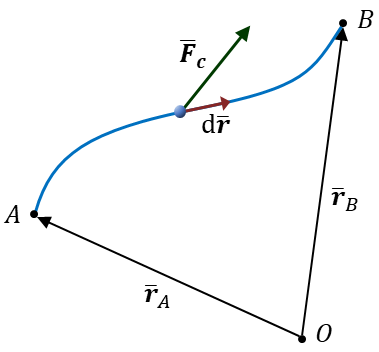
\includegraphics[width=0.34\textwidth]{figures/fig_potential-energy-01.png}
		\end{wrapfigure}
		Let us consider a particle being acted upon by a net conservative force $\vb{F}_c$ only. Then the total work done by $\vb{F}_c$ in moving an arbitrary particle from an initial point $A$ (at position $\vb{r}_A$) to a final point $B$ (at position $\vb{r}_B$) is
		\resetwrappadding
		\begin{align*}
			\int\limits_{\vb{r}_A}^{\vb{r}_B}{\vb{F}_c\cdot\dd{\vb{r}}}=\qty(\text{function of }\vb{r}_B) - \qty(\text{function of }\vb{r}_A)
		\end{align*}
		We refer to this function of position as the potential energy function $U$ and write the above equation as follows
		\begin{align*}
			\int\limits_{\vb{r}_A}^{\vb{r}_B}{\vb{F}_c\cdot\dd{\vb{r}}}=\qty[-U(\vb{r}_B)]-\qty[-U(\vb{r}_A)]
		\end{align*}
		where the negative sign on $U$ is to ensure the conservation of mechanical energy, which is observed experimentally.
		
		Hence the above equation can be written as
		\begin{align}
			\int\limits_{\vb{r}_A}^{\vb{r}_B}{\vb{F}_c\cdot\dd{\vb{r}}}=U(\vb{r}_A)-U(\vb{r}_B) \label{eqn:U-cons-F-01}
		\end{align}
		
		We assume that this potential energy function vanishes at far-off distances from the source of the conservative force, i.e. $U\to 0$ as $\vb{r}\to\infty$.
		
		Choosing $\vb{r}_A\to\infty$ and $\vb{r}_B=\vb{r}$, we obtain from equation (\ref{eqn:U-cons-F-01})
		\begin{align}
			\int\limits_{\infty}^{\vb{r}}{\vb{F}_c\cdot\dd{\vb{r}}}&=\underbrace{U(\infty)}_{=0}-U(\vb{r}) \nonumber \\
			\implies \Aboxed{U(\vb{r})&=-\int\limits_{\infty}^{\vb{r}}{\vb{F}_c\cdot\dd{\vb{r}}}} \label{eqn:U-cons-F-02}
		\end{align}
		
		Equation (\ref{eqn:U-cons-F-02}) shows that the potential energy of a particle at an arbitrary position equals the negative of the work done in moving that particle from a far-off distance to that position.

	\setcounter{equation}{0}
	\subsection{Conservative force as a negative gradient of potential energy}
		When a particle is acted upon by a net conservative force, the potential energy at an arbitrary point is a function of the position alone. So, for instance, in Cartesian coordinates we have $U(\vb{r})=U(x,y,z)$. Hence the total differential of the potential energy is
		\begin{align*}
			\dd{U}&=\pdv{U}{x}\dd{x} + \pdv{U}{y}\dd{y} + \pdv{U}{z}\dd{z}
		\end{align*}
		At far-off points, we have $U(\vb{r}\to\infty)=0$. Hence we can integrate the above from a far-off point to some arbitrary position $\vb{r}$ as follows
		\begin{align}
			U(\vb{r})&=\int\limits_{0}^{U(\vb{r})}{\dd{U}} \nonumber\\
			\implies U(\vb{r})&=\int\limits_{\infty}^{\vb{r}}{\qty[\pdv{U}{x}\dd{x} + \pdv{U}{y}\dd{y} + \pdv{U}{z}\dd{z}]} \label{eqn:U-total-diff}
		\end{align}
		We can write the net conservative force in a Cartesian system as
		\begin{align}
			\vb{F}_c&=F_x\vu{x}+F_y\vu{y}+F_z\vu{z} \label{eqn:Fc-comp}
		\end{align}
		
		Now, from the definition of the potential energy function, we have
		\begin{align}
			U(\vb{r})&=-\int\limits_{\infty}^{\vb{r}}{\vb{F}_c\cdot\dd{\vb{r}}} \nonumber\\
				&=-\int\limits_{\infty}^{\vb{r}}{\qty(F_x\vu{x}+F_y\vu{y}+F_z\vu{z})\cdot\qty(\vu{x}\dd{x}+\vu{y}\dd{y}+\vu{z}\dd{z})} \nonumber\\
			\implies U(\vb{r})&=-\int\limits_{\infty}^{\vb{r}}{\qty(F_x\dd{x}+F_y\dd{y}+F_z\dd{z})} \label{eqn:U-integ-F}
		\end{align}
		
		Comparing equations (\ref{eqn:U-total-diff}) and (\ref{eqn:U-integ-F}), we get
		\begin{align*}
			F_x=-\pdv{U}{x},\quad F_y=-\pdv{U}{y},\quad F_z=-\pdv{U}{z}
		\end{align*}
		
		Hence from equation (\ref{eqn:Fc-comp}), we obtain
		\begin{align}
			\vb{F}_c&=-\pdv{U}{x}\vu{x}-\pdv{U}{y}\vu{y}-\pdv{U}{z}\vu{z} \nonumber\\
			\implies\vb{F}_c&=-\qty[\vu{x}\pdv{x}+\vu{y}\pdv{y}+\vu{z}\pdv{z}]U \label{eqn:F-del-U-01}
		\end{align}
		
		The \emph{nabla operator} $\grad$ is a vector differential operator which is defined as
		\begin{align*}
			\grad&=\vu{x}\pdv{x}+\vu{y}\pdv{y}+\vu{z}\pdv{z}
		\end{align*}
		When $\grad$ acts on some scalar field $f(\vb{r})$, we obtain the \emph{gradient} of the field $\grad{f}$.
		
		Hence, equation (\ref{eqn:F-del-U-01}) can be written as
		\begin{align*}
			\Aboxed{\vb{F}_c(\vb{r})&=-\grad{U(\vb{r})}}
		\end{align*}
		
		Therefore, a conservative force can be expressed as the negative gradient of the potential energy.
	
	\setcounter{equation}{0}
	\subsection{Law of conservation of mechanical energy}
		Consider an arbitrary particle which is moving from an initial point $A$ to a final point $B$ (with position vectors $\vb{r}_A$ and $\vb{r}_B$ respectively) under the influence of conservative forces only. Suppose the net conservative force is $\vb{F}_c$.
		
		We know that the potential energy at an arbitrary point $\vb{r}$ is given as
		\begin{align*}
			U(\vb{r})=-\int\limits_{\infty}^{\vb{r}}{\vb{F}_c\cdot\dd{\vb{r}}}
		\end{align*}
		Then the potential energies at the positions of $A$ and $B$ are
		\begin{align*}
			U_A=-\int\limits_{\infty}^{\vb{r}_A}{\vb{F}_c\cdot\dd{\vb{r}}} \qq{and} U_B=-\int\limits_{\infty}^{\vb{r}_B}{\vb{F}_c\cdot\dd{\vb{r}}}
		\end{align*}
		Hence the change in the potential energy during the entire motion of the particle is
		\begin{align}
			\Delta U&=U_B - U_A \nonumber\\
				&=\qty[-\int\limits_{\infty}^{\vb{r}_B}{\vb{F}_c\cdot\dd{\vb{r}}}] - \qty[-\int\limits_{\infty}^{\vb{r}_A}{\vb{F}_c\cdot\dd{\vb{r}}}] \nonumber\\
				&=\qty[-\int\limits_{\infty}^{\vb{r}_B}{\vb{F}_c\cdot\dd{\vb{r}}}] - \qty[\int\limits_{\vb{r}_A}^{\infty}{\vb{F}_c\cdot\dd{\vb{r}}}] \nonumber\\
				&=-\int\limits_{\infty}^{\vb{r}_B}{\vb{F}_c\cdot\dd{\vb{r}}} - \int\limits_{\vb{r}_A}^{\infty}{\vb{F}_c\cdot\dd{\vb{r}}} \nonumber\\
				&=-\qty[\int\limits_{\vb{r}_A}^{\infty}{\vb{F}_c\cdot\dd{\vb{r}}} + \int\limits_{\infty}^{\vb{r}_B}{\vb{F}_c\cdot\dd{\vb{r}}}] \nonumber\\
			\implies\Delta U&=-\int\limits_{\vb{r}_A}^{\vb{r}_B}{\vb{F}_c\cdot\dd{\vb{r}}} \label{eqn:Delta-U-cons-eng}
		\end{align}
		
		The total work done by the conservative forces in moving the particle from $A$ to $B$ is
		\begin{align}
			W&=\int\limits_{\vb{r}_A}^{\vb{r}_B}{\vb{F}_c\cdot\dd{\vb{r}}} \label{eqn:W-tot-cons-eng}\\
			\qq{also,}W&=-\Delta U\qq{[using eqn. (\ref{eqn:Delta-U-cons-eng})]} \nonumber
		\end{align}
		
		From the work-energy theorem, we know that the total work done equals the change in kinetic energy of the particle, i.e.
		\begin{align}
			W&=\Delta T=T_B - T_A \label{eqn:Delta-T-cons-eng}
		\end{align}
		where $T_A$ and $T_B$ are the kinetic energies of the particle at points $A$ and $B$ respectively.
		
		Hence, from equations (\ref{eqn:Delta-U-cons-eng}), (\ref{eqn:W-tot-cons-eng}) and (\ref{eqn:Delta-T-cons-eng}), we obtain
		\begin{align*}
			\Delta U&=-\Delta T \\
			\implies\Delta T+\Delta U&=0 \\
			\implies\qty(T_B-T_A)+\qty(U_B-U_A)&=0 \\
			\implies T_A+U_A&=T_B+U_B \\
			\implies E_A&=E_B \\
			\implies\Aboxed{E&=\text{constant}}
		\end{align*}
		
		Therefore, the mechanical energy (which is the sum of the kinetic and potential energies) remains constant when a particle moves under the influence of conservative forces alone.
		
		This is known as the \emph{law of conservation of mechanical energy}.
	
	\setcounter{equation}{0}
	\subsection{Work done by non-conservative forces}
		Consider a particle, moving along an arbitrary path from point $A$ to point $B$, as shown below.
		\begin{figure}[h!]
			\centering
			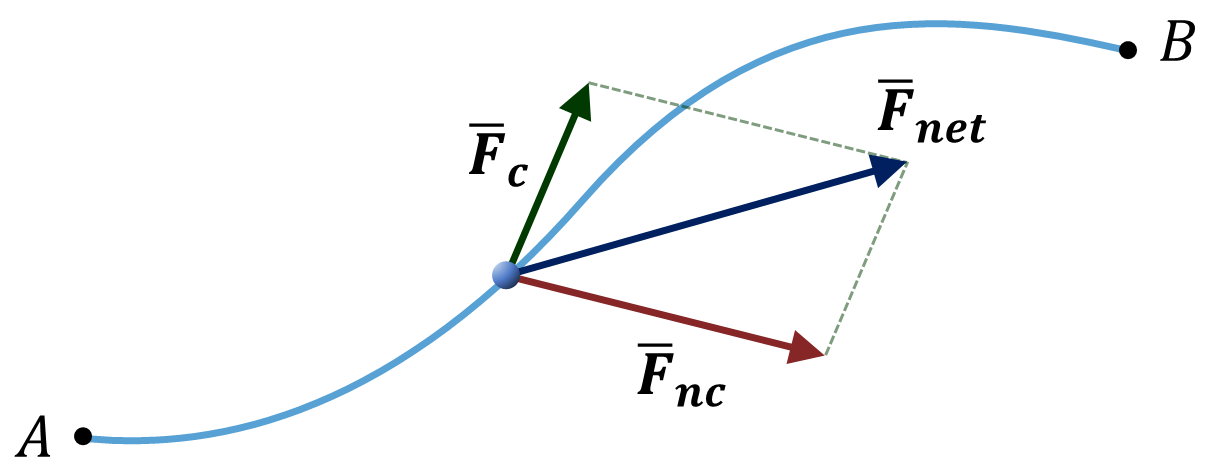
\includegraphics[width=0.5\textwidth]{figures/fig_work-non-cons.png}
		\end{figure}
		
		Suppose the resultant of all conservative forces is $\vb{F}_c$ and the resultant of all non-conservative forces is $\vb{F}_{nc}$. Then the net force acting on the particle at any point on its path is
		\begin{align}
			\vb{F}_\text{net}&=\vb{F}_c+\vb{F}_{nc} \label{eqn:F-net-Fc-Fnc}
		\end{align}
		
		Then the total work done by all the forces in moving the particle along the path is
		\begin{align}
			W_\text{total}&=\int\limits_{A}^{B}{\vb{F}_\text{net}\cdot\dd{\vb{r}}} \nonumber\\
				&=\int\limits_{A}^{B}{\qty(\vb{F}_c+\vb{F}_{nc})\cdot\dd{\vb{r}}}\qq{[using eqn. (\ref{eqn:F-net-Fc-Fnc})]} \nonumber\\
				&=\int\limits_{A}^{B}{\vb{F}_c\cdot\dd{\vb{r}}} + \int\limits_{A}^{B}{\vb{F}_{nc}\cdot\dd{\vb{r}}} \nonumber\\
			\implies W_\text{total}&=W_c+W_{nc} \label{eqn:W-tot-Wc-Wnc}
		\end{align}
		
		In equation (\ref{eqn:W-tot-Wc-Wnc}), $W_c$ and $W_{nc}$ are the work done separately on the particle by the conservative and the non-conservative forces respectively.
		
		From the work-energy theorem, the change in the kinetic energy of the particle equals the total work done on it, i.e.
		\begin{align}
			W_\text{total}&=\Delta T \label{eqn:W-T-theorem}
		\end{align}
		
		Also, the change in the potential energy of the particle equals the negative of the work done on it by the conservative forces, i.e.
		\begin{align}
			W_c&=-\Delta U \label{eqn:Delta-U-Wc}
		\end{align}
		
		Hence, from equations (\ref{eqn:W-tot-Wc-Wnc}), (\ref{eqn:W-T-theorem}) and (\ref{eqn:Delta-U-Wc}), we obtain
		\begin{align}
			\Delta T&=-\Delta U+W_{nc} \nonumber\\
			\implies W_{nc}&=\Delta T + \Delta U \nonumber\\
				&=\Delta\qty(T+U) \nonumber\\
			\implies\Aboxed{W_{nc}&=\Delta E} \label{eqn:W-nc-Del-E}
		\end{align}
		
		Therefore, the work done on a system by all the non-conservative forces equals the change in the mechanical energy of the system.
		
		This is known as the \emph{general law of conservation of energy}.
		
		\subsubsection*{Special case}
			Suppose we have a system in which non-conservative forces are either absent or do no work. In either case, we would have $W_{nc}=0$. In such a system, only the conservative forces do any work.
			
			Then from equation (\ref{eqn:W-nc-Del-E}), we obtain
			\begin{align*}
				\Delta E&=0 \\
				\implies E&=\text{constant}
			\end{align*}
			
			Therefore, this special case reduces to the law of conservation of mechanical energy.